\documentclass[11pt,a4paper]{article}
\usepackage[utf8x]{inputenc}
\usepackage[T1]{fontenc}
\usepackage{url}
\usepackage[colorlinks=true, allcolors=blue]{hyperref}
\usepackage{graphicx}
\usepackage{listings}
\usepackage{cleveref}
\crefname{lstlisting}{Listing}{Listings}
\Crefname{lstlisting}{Listing}{Listings}
\crefname{lstnumber}{Listing}{Listings}
\Crefname{lstnumber}{Listing}{Listings}
\usepackage{color}
\usepackage{wrapfig}
\usepackage{array}
\newcolumntype{P}[1]{>{\raggedright\arraybackslash}p{#1}}


\definecolor{bluekeywords}{rgb}{0.13, 0.19, 0.7}
\definecolor{greencomments}{rgb}{0.1, 0.5, 0.2}
\definecolor{redstrings}{rgb}{0.8, 0.15, 0.1}
\definecolor{graynumbers}{rgb}{0.5, 0.5, 0.5}
\definecolor{subtlegray}{rgb}{0.98, 0.98, 0.98}
\definecolor{lightgray}{rgb}{0.98, 0.98, 0.98}
\usepackage{lstautogobble}
\lstset{
    autogobble,
    columns=fullflexible,
    showspaces=false,
    showtabs=false,
    breaklines=true,
    numbers=left,
    showstringspaces=false,
    breakatwhitespace=true,
    escapeinside={(*@}{@*)},
    rulecolor=\color{lightgray},
    backgroundcolor=\color{subtlegray},
    commentstyle=\color{greencomments},
    keywordstyle=\color{bluekeywords},
    stringstyle=\color{redstrings},
    numberstyle=\color{graynumbers},
    basicstyle=\ttfamily\linespread{1.15}\footnotesize,
    frame=tb,
    framesep=12pt,
    framexleftmargin=12pt,
    tabsize=4,
    captionpos=b,
}
\graphicspath{{figures}}

\usepackage{mathptmx} % Use Times Font

\usepackage{geometry}
 \geometry{
 a4paper,
 total={170mm,257mm},
 left=20mm,
 top=20mm,
 }

\usepackage{bibentry}
\nobibliography*

\title{Cloud Systems AE1 Report}

\author{
  % Just did alphabetical order, but you're free to change if you want
  Alistair Johnston \\  2560836j
  \and
  Stefan Vučković \\ 2621177v
}

\date{{}}

\begin{document}


\flushbottom
\maketitle
\thispagestyle{empty}

\section*{Application context}
The application being considered is `a multiplayer online game by hobbyist game developers for a game jam'. For example a set of students produced an online multiplier game over 2 days as a part of Duck Sauce Game Jam 2025.

This application requires:
\begin{enumerate}
\item{Low network latency, the round trip time (RTT) should be minimised};
\item{Reliable networking, the server should have the lowest rate of packet loss possible};
\item{High network throughput, the server must be able to process many users at once without slowdown}.
\end{enumerate}

For this application the developers are students who have access to the free and student tiers of \href{https://aws.amazon.com/free/}{AWS}, \href{https://azure.microsoft.com/en-us/free/students}{Azure} and \href{https://cloud.google.com/free?hl=en}{GCP}. The developers want to compare these offerings to each other to decide which offering would best support their game.

\section*{Methodology}
For each cloud provider (AWS, Azure, GCP):
\begin{enumerate}
  \item{Deploy a VM in the `UK South' region;}
  \item{Allow 5 minutes to elapse to mitigate potential warm-up effects;}
  \item{Build and run the Go benchmarking server (\Cref{benchmarking-server}) on the VM.}
\end{enumerate}

After the VM is provisioned and warm-up effects have occurred the benchmarking can happen, on a local machine the following steps are performed:
\begin{enumerate}
  \item{Run \texttt{ping -c 200 <VM ip> > <result\_file>}, to create a log of 200 round trip times, these can then be used with the plotting script presented in \Cref{boxplot-script} to produce a boxplot of VM RTTs;}
    \item{Run Prometheus locally with the target(s) set to the IPs of the VM(s);}
    \item{Run Grafana locally and configure the Prometheus instance as a data source;}
  \item{Run the test script (shown in \Cref{test-script}) to produce metrics;}
  \item{Use Grafana to plot metrics, here we consider those defined below.}
\end{enumerate}

\begin{center}
  \begin{tabular}{P{0.2\linewidth} | P{0.8\linewidth}}
    Metric & PromQL expression \\
    \hline

Latency (per provider) & rate(network\_latency\_seconds\_sum[1m]) / rate(network\_latency\_seconds\_count[1m]) \\
Latency Variability & (max by (provider) (rate(network\_latency\_seconds\_sum[1m]) / rate(network\_latency\_seconds\_count[1m])) - min by (provider) (rate(network\_latency\_seconds\_sum[1m]) / rate(network\_latency\_seconds\_count[1m]))) \\

    \hline
Download Throughput (per provider) & rate(network\_throughput\_bytes\_total{direction="download"}[1m]) \\
Download Variability & (max by (provider) (rate(network\_throughput\_bytes\_total{direction="download"}[1m])) - min by (provider) (rate(network\_throughput\_bytes\_total{direction="download"}[1m]))) \\

    \hline
Upload Throughput (per provider) & rate(network\_throughput\_bytes\_total{direction="upload"}[1m]) \\
Upload Variability & (max by (provider) (rate(network\_throughput\_bytes\_total{direction="upload"}[1m])) - min by (provider) (rate(network\_throughput\_bytes\_total{direction="upload"}[1m]))) \\

  \end{tabular}
\end{center}

\section*{Results}

\begin{figure}
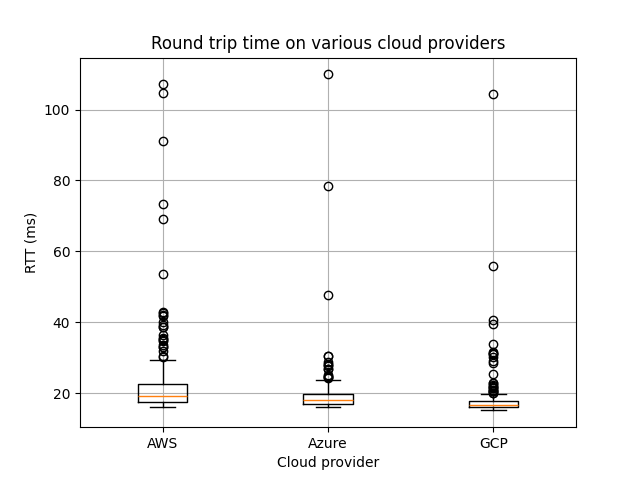
\includegraphics[width=\textwidth]{boxplot.png}
\caption{Box and whisker plot showing the round trip times for each VM}
\label{boxplot}
\end{figure}

\begin{figure}
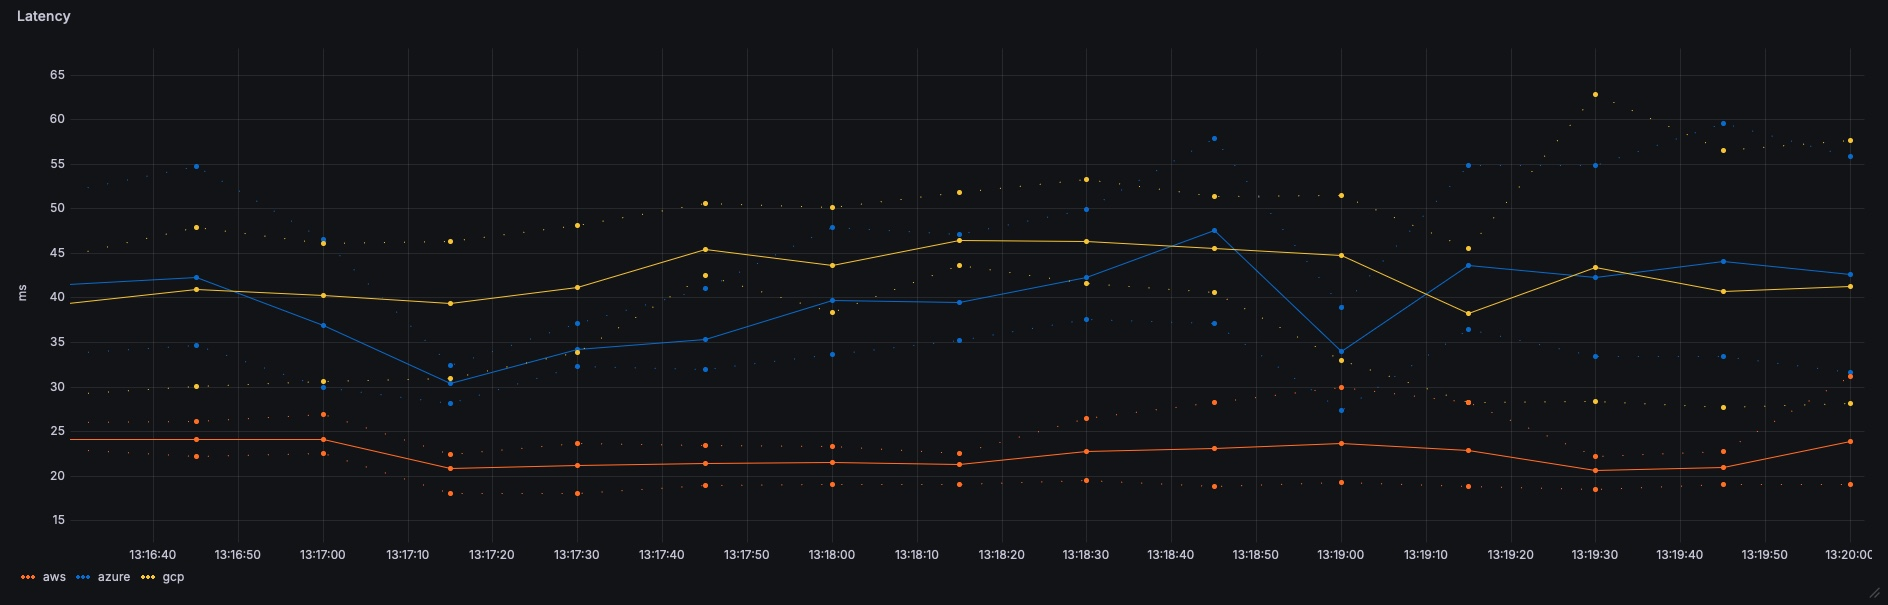
\includegraphics[width=\textwidth]{Latency.jpeg}
\caption{Grafana plot of network latency for each VM}
\label{latency}
\end{figure}

\begin{figure}
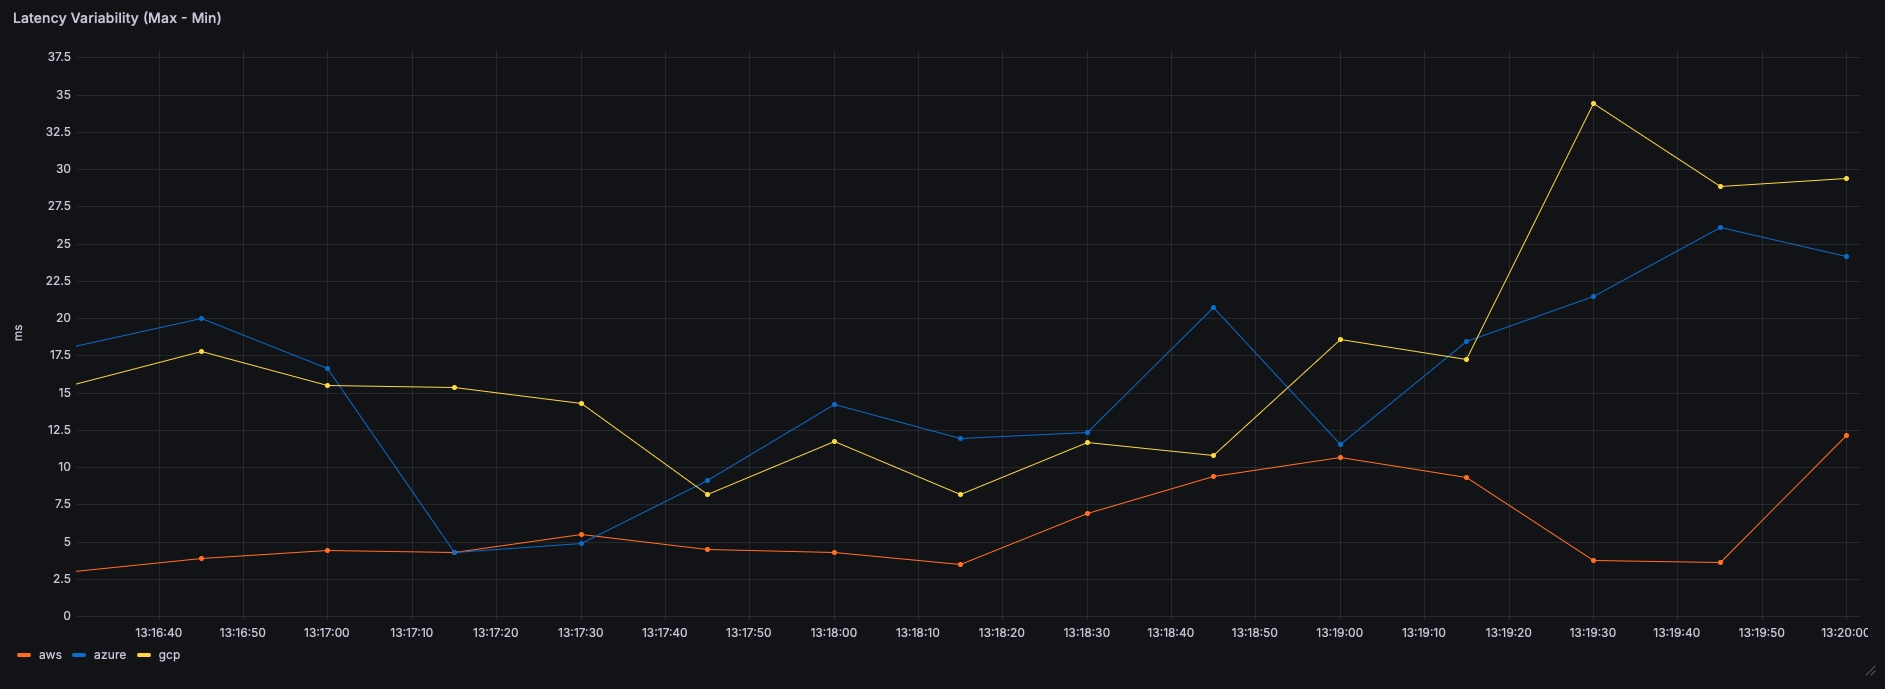
\includegraphics[width=\textwidth]{LatencyVar.jpeg}
\caption{Grafana plot of the variability of the network latency for each VM}
\label{latencyvar}
\end{figure}

\Cref{boxplot} shows the RTTs from each cloud provider, here we see that GCP outperforms both AWS and Azure. GCP has less variance and fewer outliers above 40ms, however the RTTs for the other providers have similar lows and mean RTT. While GCP has lower RTT than the other providers, \Cref{latency} shows that AWS has consistently lower network latency than both Azure and GCP. As the RTT for GCP was slightly lower than AWS this must mean that the traffic returning from AWS is much slower than traffic returning from GCP. This would be bad for the game as players rely on feedback from the server for the game to feel responsive and to inform future gameplay decisions. Unfortunately the variability for the latency on GCP is far more inconsistent than the variability experienced with the alternate VMs, spiking near the end of the test to over 3 times its lowest variability (shown in \Cref{latencyvar}). Inconsistent latency would cause jitters in gameplay which could ruin the experience for players. This would likely mean that, despite the slower RTT AWS would be the best option purely from a network latency standpoint as its RTTs are mostly comparable to GCP's but AWS has consistently lower variance. Azure is stuck in the middle of GCP and AWS with higher RTT than GCP but higher latency and variance than AWS. % this means that, only taking latency/RTT into account, AWS would be the best option for deploying a game.

\begin{figure}
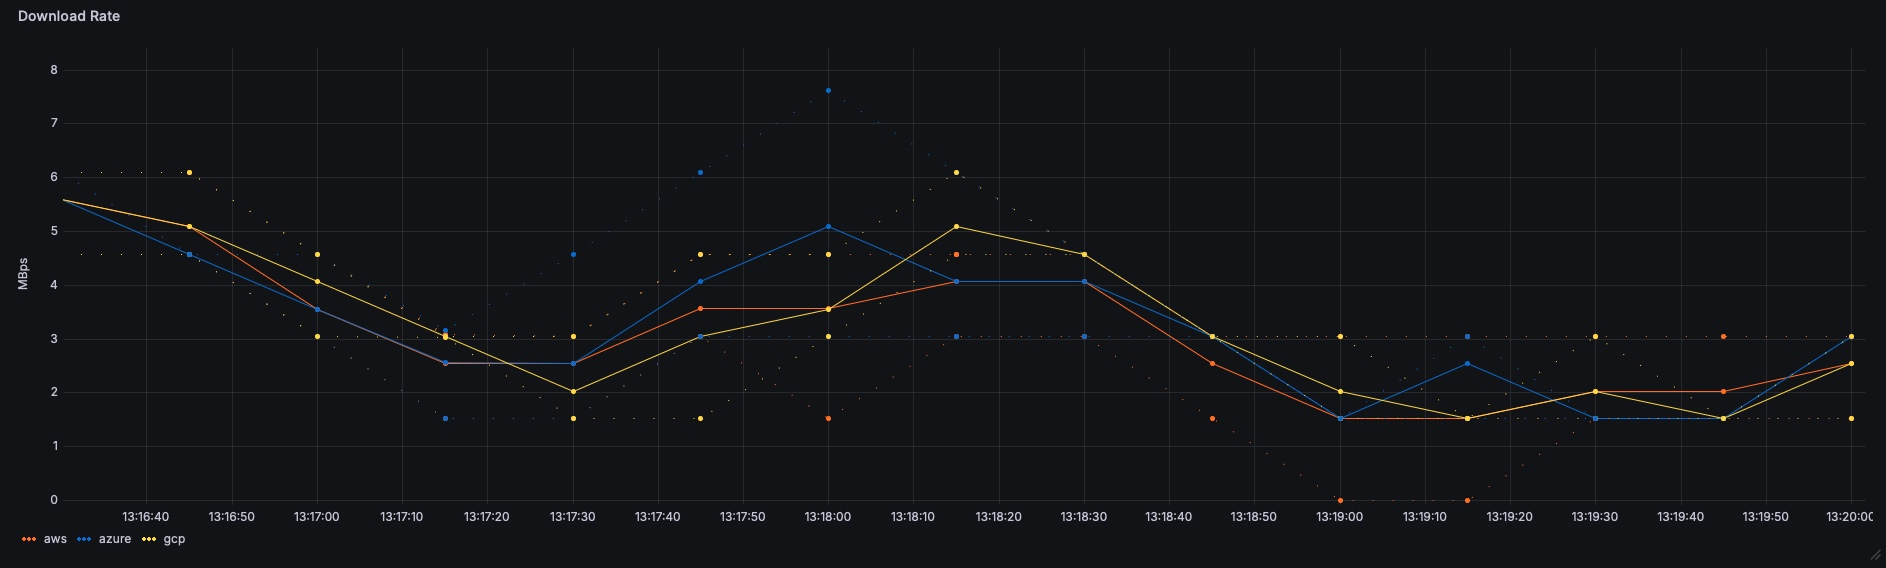
\includegraphics[width=\textwidth]{DownloadRate.jpeg}
\caption{Grafana plot of download rate for each VM}
\label{download}
\end{figure}

\begin{figure}
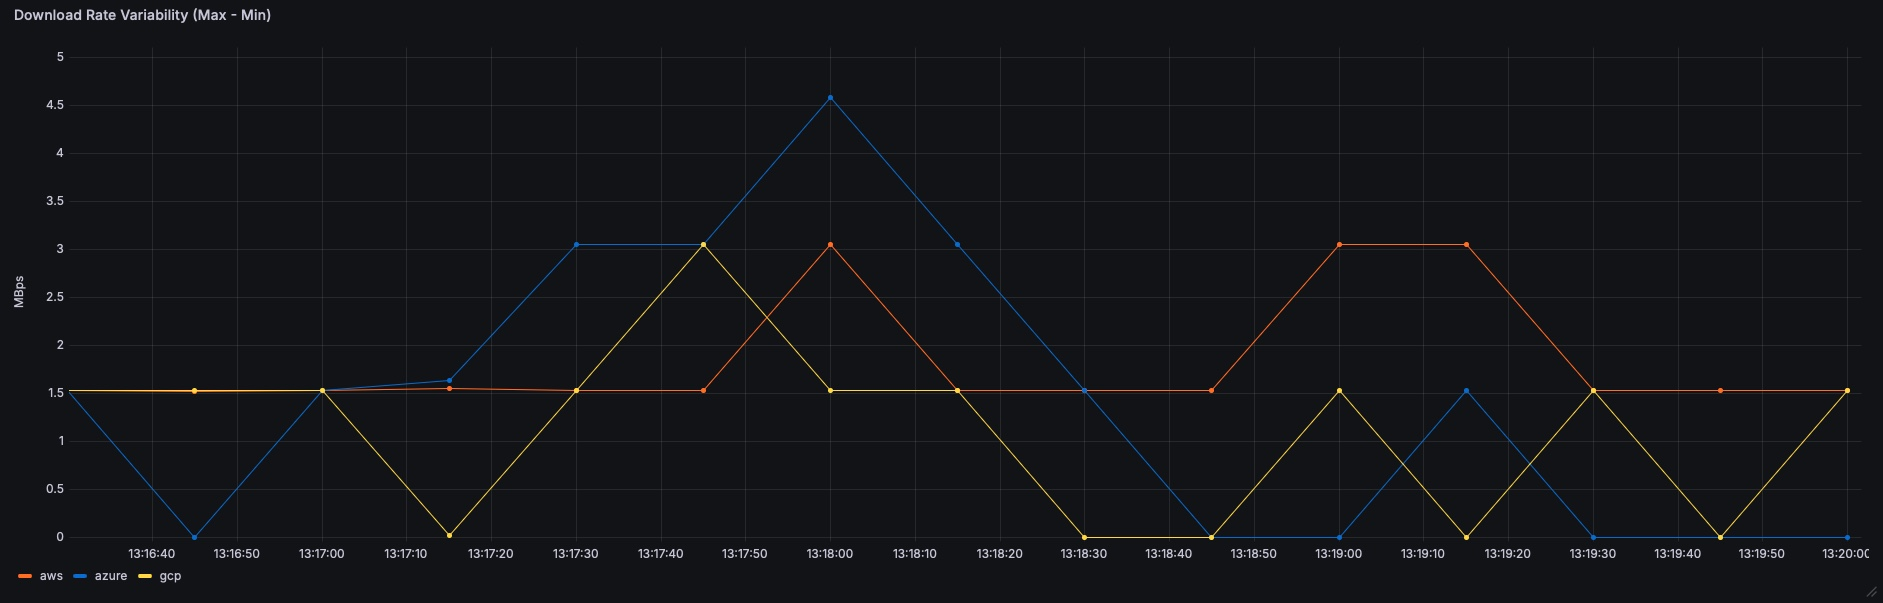
\includegraphics[width=\textwidth]{DownloadRateVar.jpeg}
\caption{Grafana plot of variability of download rate for each VM}
\label{downloadvar}
\end{figure}

\begin{figure}
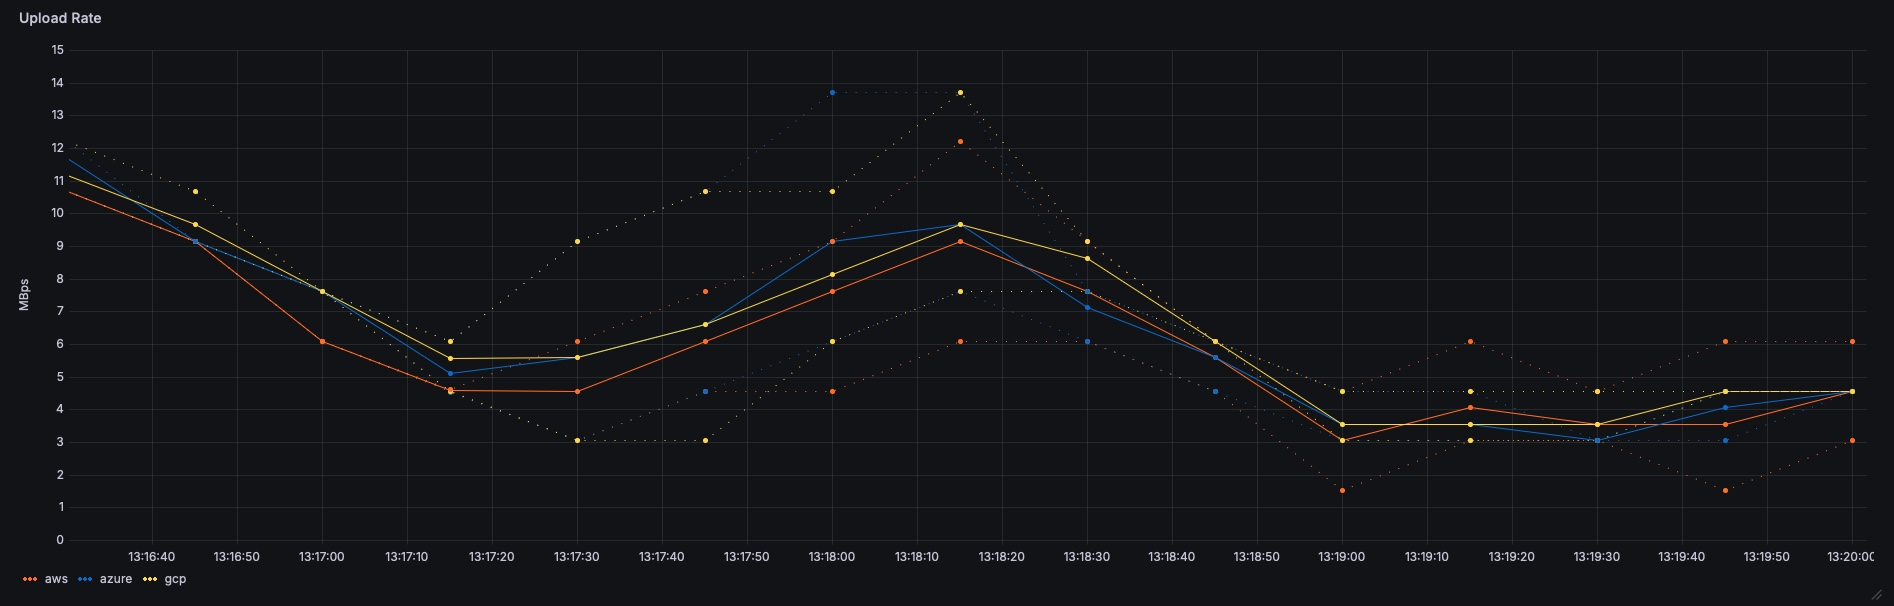
\includegraphics[width=\textwidth]{UploadRate.jpeg}
\caption{Grafana plot of upload rate for each VM}
\label{upload}
\end{figure}

\begin{figure}
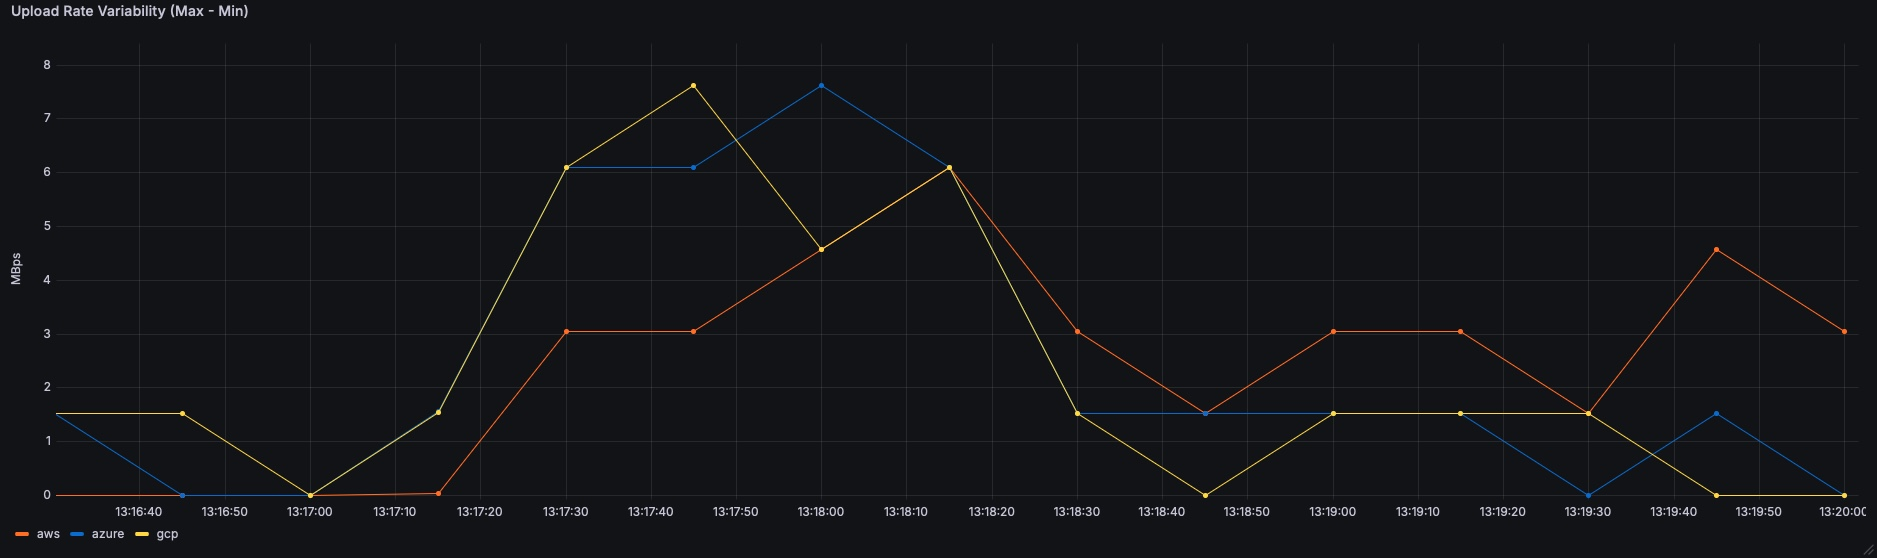
\includegraphics[width=\textwidth]{UploadRateVar.jpeg}
\caption{Grafana plot of variability of upload rate for each VM}
\label{uploadvar}
\end{figure}

Download and upload rates are mostly indistinguishable between all 3 cloud providers (shown in \Cref{download} and \Cref{upload}) with AWS potentially having slightly lower rates than the others. As this is the case for the rate itself the most important thing to look at is the rate variability. For downloads we see that Azure has the highest spike but also has periods of very low variability, while AWS and GCP have the same highs with GCP having consistently lower variability than AWS. Meanwhile the upload rates fluctuate much more heavily than downloads; Azure and GCP hit \textasciitilde 7.5MBps with AWS not far behind at a peak of \textasciitilde 6.5MBps.

\section*{Conclusions}

With the upload and download rates being extremely similar between providers and the RTT also being comparable the latency is the deciding factor for choosing between providers for the application. To this end AWS is likely the best choice for deploying the game, it has similar or lower network variability to the other providers but provides a substantially lower network latency which would lead to a more enjoyable experience.

\section*{Appendices}

\subsection*{Code Listings}
\lstinputlisting[caption=Test script, language=bash, label=test-script]{scripts/test.sh}

\lstinputlisting[caption=Benchmarking server, language=Go, label=benchmarking-server]{scripts/main.go}

\lstinputlisting[caption=Box plot for RTT, language=Python, label=boxplot-script]{scripts/ping_boxplot.py}

\end{document}
